\newif\ifalone
\alonefalse
\ifalone
\documentclass{article}
\usepackage{graphicx}
\usepackage{natbib}
\usepackage{amsfonts}
\usepackage{amssymb}
\usepackage{amsthm}
\usepackage{bm}
\usepackage{Sweave}
\usepackage{lscape}
\usepackage{makeidx}
\usepackage{hyperref}

\let\proglang=\textsf
\newcommand{\pkg}[1]{{\fontseries{b}\selectfont #1}}
  \hypersetup{%
    hyperindex = {true},
    colorlinks = {true},
    linktocpage = {true},
    plainpages = {false},
    linkcolor = {blue},
    citecolor = {blue},
    urlcolor = {red},
    pdfstartview = {Fit},
    pdfpagemode = {UseOutlines},
    pdfview = {XYZ null null null}
  }


\title{Pedigrees and Phylogenies}

\author{Jarrod Hadfield (\texttt{j.hadfield@ed.ac.uk})}
\begin{document}
\maketitle
\else
\chapter{Pedigrees and Phylogenies}
\label{chap6}
\fi



Pedigrees and phylogenies are similar things: they are both ways of representing shared ancestry. Under a quantitative genetic model of inheritance, or a Brownian motion model of evolution, GLMM's can be readily extended to model the similarities that exist between the phenotypes of related individuals or taxa.  In the context of quantitative genetics these models are known as `animal' models \citep{Henderson.1976}, and in the context of the comparative method these models are known as phylogenetic mixed models \citep{Lynch.1991}. The two models are almost identical, and are relatively minor modifications to the basic mixed model \citep{Hadfield.2010b}. 

\section{Pedigree and phylogeny formats}

\subsection{Pedigrees}

\texttt{MCMCglmm} handles pedigrees stored in 3-column tabular form, with each row representing a single individual. The first column should contain the unique identifier of the individual, and columns 2 and 3 should be the unique identifiers of the individual's parents. Parents must appear before their offspring in the table. I usually have the dam (mother) in the first column and the sire (father) in the third. I prefer the words dam and sire because if I subscript things with $m$ and $f$ I can never remember whether I mean male and female, or mother and father. In hermaphrodite systems the same individual may appear in both columns, even within the same row if an individual was produced through selfing.  This is not a problem, but \texttt{MCMCglmm} will issue a warning in case hermaphrodites are not present and a data entry mistake has been made. Impossible pedigrees (for example individual's that give birth to their own mother) are a problem and \texttt{MCMCglmm} will issue an error, hopefully with an appropriate message, when impossibilities are detected.\\

   If the parent(s) of an individual are unknown then a missing value (\texttt{NA}) should be assigned in the relevant column. All individuals appearing as dams or sires need to have their own record, even if both of their parents are unknown. Often the number of individuals in a pedigree will be greater than the number of individuals for which phenotypic data exist. \texttt{MCMCglmm} can handle this, as long as all the individuals appearing in the data frame passed to \texttt{data} also appear in the pedigree.\\
   
To illustrate, we can load a pedigree for a population of blue tits and display the pedigree for the nuclear family that has individuals \texttt{"R187920"} and \texttt{"R187920"} as parents:

\begin{Schunk}
\begin{Sinput}
> data(BTped)
> Nped <- BTped[which(apply(BTped, 1, function(x) {
+     any(x == "R187920" | x == "R187921")
+ })), ]
> Nped
\end{Sinput}
\begin{Soutput}
      animal     dam    sire
66   R187920    <NA>    <NA>
172  R187921    <NA>    <NA>
325  R187726 R187920 R187921
411  R187724 R187920 R187921
503  R187723 R187920 R187921
838  R187613 R187920 R187921
932  R187612 R187920 R187921
1030 R187609 R187920 R187921
\end{Soutput}
\end{Schunk}

Both parents form part of what is known as the base population - they are outbred and unrelated to anybody else in the pedigree.\\

\texttt{MCMCglmm} and \texttt{MasterBayes} have several pedigree manipulation functions. (\texttt{MasterBayes::orderPed})  orders a pedigree so parents appear before their offspring, (\texttt{MasterBayes::insertPed}) inserts records for individuals that only appear as parents (or a vector of specified individuals).  When the number of individuals with phenotypic data is less than the number of individuals in the pedigree it is sometimes possible to remove uninformative individuals from the pedigree and thus reduce the computation time. This is known as pruning the pedigree and is implemented in the  \texttt{MCMCglmm} function \texttt{prunePed}. A vector of measured individuals is specified in the argument \texttt{keep} and specifying \texttt{make.base=TRUE} implements the most complete pruning. Note,  \texttt{make.base=FALSE} is the default argument so you'll need to explicitly specify \texttt{TRUE} in the call to  \texttt{prunePed}. Michael Morrissey's \texttt{pedantics} package, and the \texttt{kinship} package also have many other useful pedigree orientated functions. In fact, the \texttt{orderPed} function in \texttt{MasterBayes} is built around functions provided by  \texttt{kinship}.\\

\subsection{Phylogenies}

Phylogenies can be expressed in tabular form, although only two columns are required because each species only has a single parent. In general however,  phylogenies are not expressed in this form presumably because it is hard to traverse phylogenies (and pedigrees) backwards in time when they are stored this way. For phylogenetic mixed models we generally only need to traverse phylogenies forward in time (if at all) but I have stuck with convention and used the \texttt{phylo} class from the \texttt{ape} package to store phylogenies.  As with pedigrees, all species appearing in the data frame passed to \texttt{data} need to appear in the phylogeny. Typically, this will only include species at the tips of the phylogeny and so the measured species should appear in the \texttt{tip.label} element of the phylo object. An error message will be issued if this is not the case. Data may also exist for ancestral species, or even for species present at the tips but measured many generations before. It is possible to include these data as long as the phylogeny has labelled internal nodes. If nodes are unlabeled then  \texttt{MCMCglmm}  names them internally using the default arguments of   \texttt{makeNodeLabel} from \texttt{ape}.\\ 

To illustrate, lets take the phylogeny of bird families included in the \texttt{ape} package, and extract the phylogeny in tabular form for the Paridae (Tits), Certhiidae (Treecreepers), Gruidae (Cranes) and the Struthionidae (Ostriches):

\begin{Schunk}
\begin{Sinput}
> data("bird.families")
> bird.families <- makeNodeLabel(bird.families)
> some.families <- c("Certhiidae", "Paridae", "Gruidae", "Struthionidae")
> Nphylo <- drop.tip(bird.families, setdiff(bird.families$tip.label, 
+     some.families))
> INphylo <- inverseA(Nphylo)
> INphylo$pedigree
\end{Sinput}
\begin{Soutput}
     node.names                  
[1,] "Node58"        NA        NA
[2,] "Node122"       "Node58"  NA
[3,] "Struthionidae" NA        NA
[4,] "Gruidae"       "Node58"  NA
[5,] "Certhiidae"    "Node122" NA
[6,] "Paridae"       "Node122" NA
\end{Soutput}
\end{Schunk}



\begin{figure}[!h]
\begin{center}
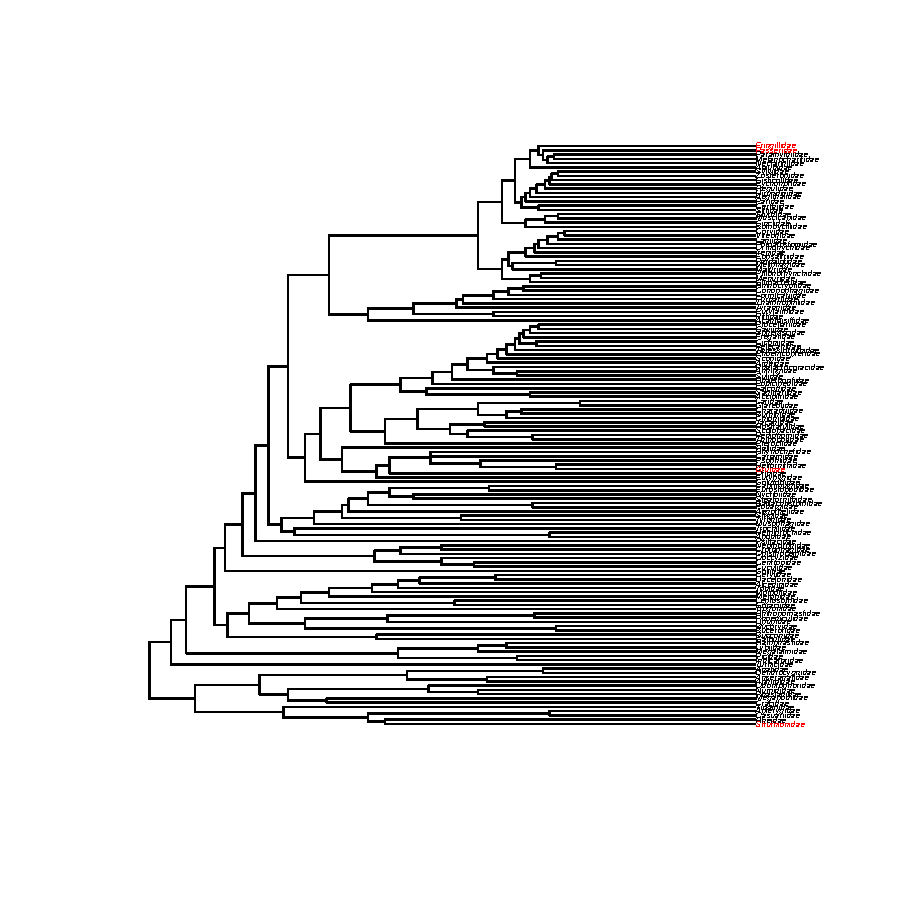
\includegraphics{Lecture6-005}
\end{center}
\caption{A phylogeny of bird families from \citet{Sibley.1990} The families in red are the Tits (Paridae), Treecreepers (Certhiidae),  Cranes (Gruidae)  and the Ostriches (Struthionidae) from top to bottom. Blue tits are in the Paridae, and the word pedigree comes from the french for crane's foot.}
\label{bird.families-fig}
\end{figure}

 The full phylogeny, with these families and their connecting notes displayed, is shown in Figure \ref{bird.families-fig}. You will notice that \texttt{Node1} - the root - does not appear in the phylogeny in tabular form. This is because the root is equivalent to the base population in a pedigree analysis, an issue which we will come back to later. Another piece of information that seems to be lacking in the tabular form is the branch length information. Branch lengths are equivalent to inbreeding coefficients in a pedigree. As with pedigrees the inbreeding coefficients are calculated by \texttt{inverseA}:
 
\begin{Schunk}
\begin{Sinput}
> INphylo$inbreeding
\end{Sinput}
\begin{Soutput}
[1] 0.2285714 0.3857143 1.0000000 0.7714286 0.3857143 0.3857143
\end{Soutput}
\end{Schunk}

You will notice that the Struthionidae have an inbreeding coefficient of 1 because we used the default \texttt{scale=TRUE} in the call to \texttt{inverseA}.  Only ultrametric trees can be scaled in \texttt{MCMCglmm} and in this case the sum of the inbreeding coefficients connecting the root to a terminal node is one. To take the Paridae as an example:

\begin{Schunk}
\begin{Sinput}
> sum(INphylo$inbreeding[which(INphylo$pedigree[, 1] %in% c("Paridae", 
+     "Node122", "Node58"))])
\end{Sinput}
\begin{Soutput}
[1] 1
\end{Soutput}
\end{Schunk}

The inbreeding coefficients for the members of the blue tit nuclear family are of course all zero:

\begin{Schunk}
\begin{Sinput}
> inverseA(Nped)$inbreeding
\end{Sinput}
\begin{Soutput}
[1] 0 0 0 0 0 0 0 0
\end{Soutput}
\end{Schunk}

\section{The animal model and the phylogenetic mixed model}

The structure of pedigrees and phylogenies can be expressed in terms of the relatedness matrix  ${\bf A}$. This matrix is symmetric, square, and has dimensions equal to the number of individuals in the pedigree (or the number of taxa in the phylogeny). For pedigrees, element $A_{i,j}$ is twice the probability that an allele drawn from individual $i$ is identical by descent to an allele in individual $j$.  For phylogenies, element $A_{i,j}$ is the amount of time that elapsed (since the common ancestor of all sampled taxa) before the speciation event that resulted in taxa $i$ and $j$. Simple, but perhaps slow, recursive methods exist for calculating  ${\bf A}$ in both cases:

\begin{Schunk}
\begin{Sinput}
> Aped <- 2 * kinship::kinship(Nped[, 1], Nped[, 2], Nped[, 3])
> Aped
\end{Sinput}
\begin{Soutput}
        R187920 R187921 R187726 R187724 R187723 R187613 R187612 R187609
R187920     1.0     0.0     0.5     0.5     0.5     0.5     0.5     0.5
R187921     0.0     1.0     0.5     0.5     0.5     0.5     0.5     0.5
R187726     0.5     0.5     1.0     0.5     0.5     0.5     0.5     0.5
R187724     0.5     0.5     0.5     1.0     0.5     0.5     0.5     0.5
R187723     0.5     0.5     0.5     0.5     1.0     0.5     0.5     0.5
R187613     0.5     0.5     0.5     0.5     0.5     1.0     0.5     0.5
R187612     0.5     0.5     0.5     0.5     0.5     0.5     1.0     0.5
R187609     0.5     0.5     0.5     0.5     0.5     0.5     0.5     1.0
\end{Soutput}
\end{Schunk}

\begin{Schunk}
\begin{Sinput}
> Aphylo <- vcv.phylo(Nphylo, cor = T)
> Aphylo
\end{Sinput}
\begin{Soutput}
              Struthionidae   Gruidae Certhiidae   Paridae
Struthionidae             1 0.0000000  0.0000000 0.0000000
Gruidae                   0 1.0000000  0.2285714 0.2285714
Certhiidae                0 0.2285714  1.0000000 0.6142857
Paridae                   0 0.2285714  0.6142857 1.0000000
\end{Soutput}
\end{Schunk}

Note that specifying \texttt{cor=T} is equivalent to scaling the tree as we did in the argument to \texttt{inverseA}.\\

In fact, all of the mixed models we fitted in earlier sections also used an ${\bf A}$ matrix, but in those cases the matrix was an identity matrix ${\bf I}$ and we didn't have to worry about it. Let's reconsider the Blue tit model \texttt{m3a.1} from Section \ref{chap3} where we were interested in estimating \texttt{sex} effects for \texttt{tarsus} length together with the amount of variance explained by genetic mother (\texttt{dam}) and  foster mother  (\texttt{fosternest}):

\begin{Schunk}
\begin{Sinput}
> m3a.1 <- MCMCglmm(tarsus ~ sex, random = ~dam + fosternest, data = BTdata, 
+     verbose = FALSE, prior = prior)
\end{Sinput}
\end{Schunk}

 All individuals that contributed to that analysis are from a single generation and appear in \texttt{BTped} together with their parents. However, individuals in the parental generation do not have tarsus length measurements so they do not have their own records in \texttt{BTdata}.\\

The model can be expressed as:

\begin{equation}
{\bf y}  = {\bf X}{\bm \beta}+{\bf Z}_{1}{\bf u}_{1}+{\bf Z}_{2}{\bf u}_{2}+{\bf e}
\end{equation}

where the design matrices contain information relating each individual to a  \texttt{sex} (${\bf X}$) a  \texttt{dam} (${\bf Z}_{1}$) and a \texttt{fosternest}(${\bf Z}_{2}$). The associated parameter vectors (${\bm \beta}$, ${\bf u}_{1}$ and ${\bf u}_{2}$) are the effects of each \texttt{sex}, \texttt{mother} and \texttt{fosternest} on \texttt{tarsus} length, and ${\bf e}$ is the vector of residuals.\\

In the model, the $u$'s are treated as random so we estimate their variance instead of fixing it in the prior at some (large) value, as we did with the $\beta$'s.  We can be a little more explicit about what this means:

\begin{equation}
{\bf u}_{1}  \sim N({\bf 0},\ {\bf I}\sigma^{2}_{1})
\end{equation}

where $\sim$ stands for `is distributed as' and $N$ a (multivariate) normal distribution. The distribution has two sets of parameters; a vector of means and a covariance matrix. We assume the random effects are deviations around the fixed effect part of the model and so they have a prior expectation  of zero. The (co)variance matrix of the random effects is ${\bf I}\sigma^{2}_{1}$ where $\sigma^{2}_{1}$ is the variance component to be estimated.  The use of the identity matrix makes two things explicit. First, because all off-diagonal elements of an identity matrix are zero we are assuming that all \texttt{dam} effects are independent (no covariance exists between any two \texttt{dam} effects). Second, all diagonal elements of an identity matrix are 1 implying that the range of possible values the dam effect \emph{could} take is equivalent for every \texttt{dam}, this range being governed by the magnitude of the variance component.\\

Since \texttt{dam}'s have very little interaction with the subset of offspring that were moved to a \texttt{fosternest}), we may be willing to assume that any similarity that exists between the tarsus lengths of this susbset and the subset  that remained at home must be due to genetic effects.   although not strictly true we can assume that individuals that shared the same dam also shared the same sire, and so share around \%50 of their genes.    

\ifalone
\bibliographystyle{jss}
\bibliography{JarLib}
\end{document}
\else
\fi

